\documentclass[12pt]{article}
\usepackage[spanish]{babel}
\usepackage[a4paper, margin=1in]{geometry}
\usepackage{xcolor}
\usepackage{float}
\usepackage{graphicx}

\definecolor{darkblue}{RGB}{31, 78, 120}
\definecolor{lightblue}{RGB}{46, 117, 182}
\definecolor{gray}{RGB}{89, 89, 89}

\pagestyle{empty}
\setlength{\parindent}{0pt}

\begin{document}

\vspace*{0.5cm}
\begin{center}
    \textcolor{lightblue}{\textbf{\fontsize{26}{31}\selectfont PAFP}}
\end{center}
\vspace{0.8cm}
\begin{center}
    \textcolor{lightblue}{\rule{6cm}{2pt}}
\end{center}
\vspace{1cm}
\begin{center}
    \textit{\fontsize{16}{19}\selectfont \textcolor{gray}{Informe de Tesis}}
\end{center}
\vspace{1cm}
\begin{center}
    \textbf{\fontsize{12}{14}\selectfont Autor:}
\end{center}
\begin{center}
    \fontsize{12}{14}\selectfont Laura Juliana Garzon Arias\\[2pt]
    \fontsize{12}{14}\selectfont Juan felipe Romero Ortiz\\[2pt]
    \fontsize{12}{14}\selectfont Xiomara Herrera Suárez\\[2pt]
    \fontsize{12}{14}\selectfont Sebastian Almanza Galvis
\end{center}
\vspace{0.8cm}
\begin{center}
    \textbf{\fontsize{12}{14}\selectfont Institución:}
\end{center}
\begin{center}
    \fontsize{12}{14}\selectfont Pontificia universidad javeriana
\end{center}
\vspace{0.8cm}
\begin{center}
    \textbf{\fontsize{12}{14}\selectfont Director de Tesis:}
\end{center}
\begin{center}
    \fontsize{12}{14}\selectfont Cecile Eugenie Gloria Gauthier Umaña
\end{center}
\vspace{1.5cm}
\begin{center}
    \textcolor{gray}{\fontsize{12}{14}\selectfont Bogotá, Colombia}
\end{center}
\begin{center}
    \textcolor{gray}{\fontsize{12}{14}\selectfont abril 2026 }
\end{center}

\newpage

% =============================================
\section{Comentarios 1: Andrea Rueda}
% =============================================

\begin{figure}[H]
    \centering
    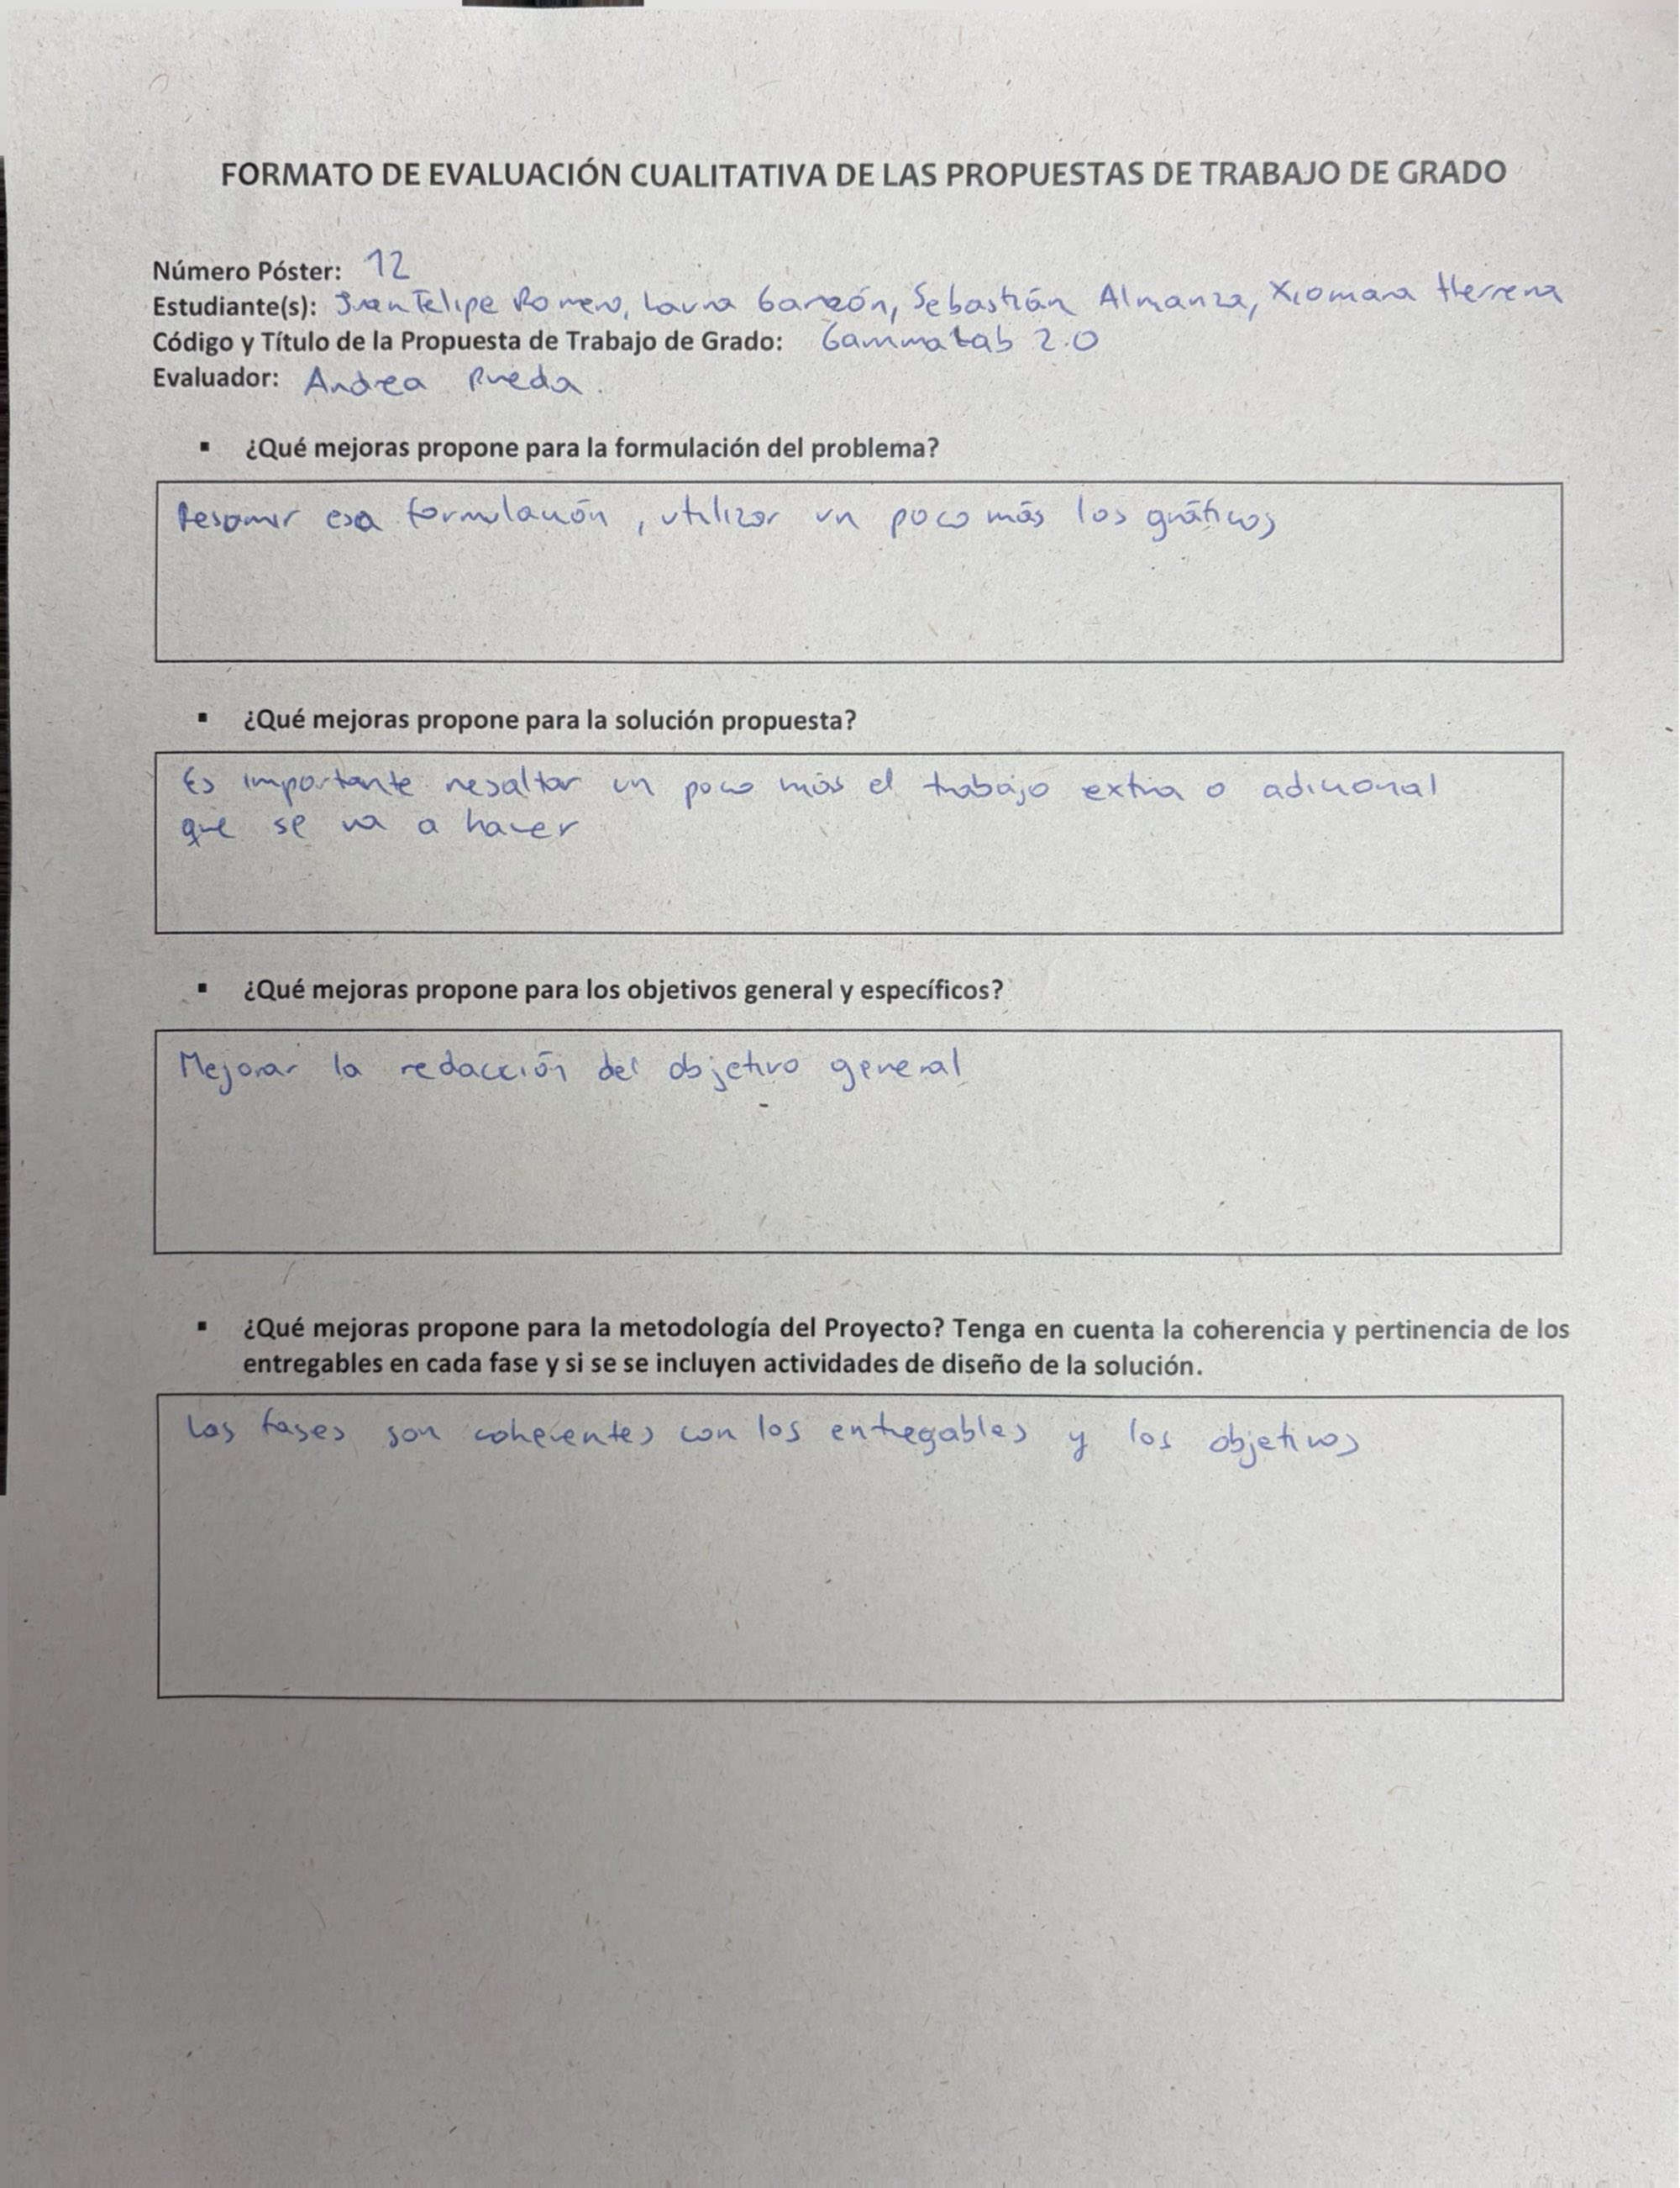
\includegraphics[width=0.9\linewidth]{andrea 1.png}
    \caption{Ejemplo de comentario}
    \label{fig:andrea1}
\end{figure}

\textbf{\textcolor{darkblue}{Respuesta a los comentarios de Andrea Rueda:}}\\[6pt]

\textbf{Formulación del problema:} Agradecemos la sugerencia de incorporar más elementos gráficos. Procederemos a enriquecer esta sección con diagramas y figuras que ilustren el contexto y la magnitud del problema de manera más visual y comprensible.\\[4pt]

\textbf{Solución propuesta:} Aceptamos plenamente la observación. Ampliaremos la descripción de la solución para destacar con mayor claridad el trabajo adicional y los aportes nuevos que distinguen este proyecto de versiones o trabajos previos relacionados.\\[4pt]

\textbf{Objetivos general y específicos:} Tomamos nota de la necesidad de mejorar la redacción del objetivo general. Lo reformularemos para que sea más preciso, medible y coherente con el alcance real del proyecto.\\[4pt]

\textbf{Metodología:} Agradecemos la valoración positiva sobre la coherencia entre fases, entregables y objetivos. Mantendremos esta alineación y la reforzaremos con mayor detalle en la descripción de cada fase.

\begin{figure}[H]
    \centering
    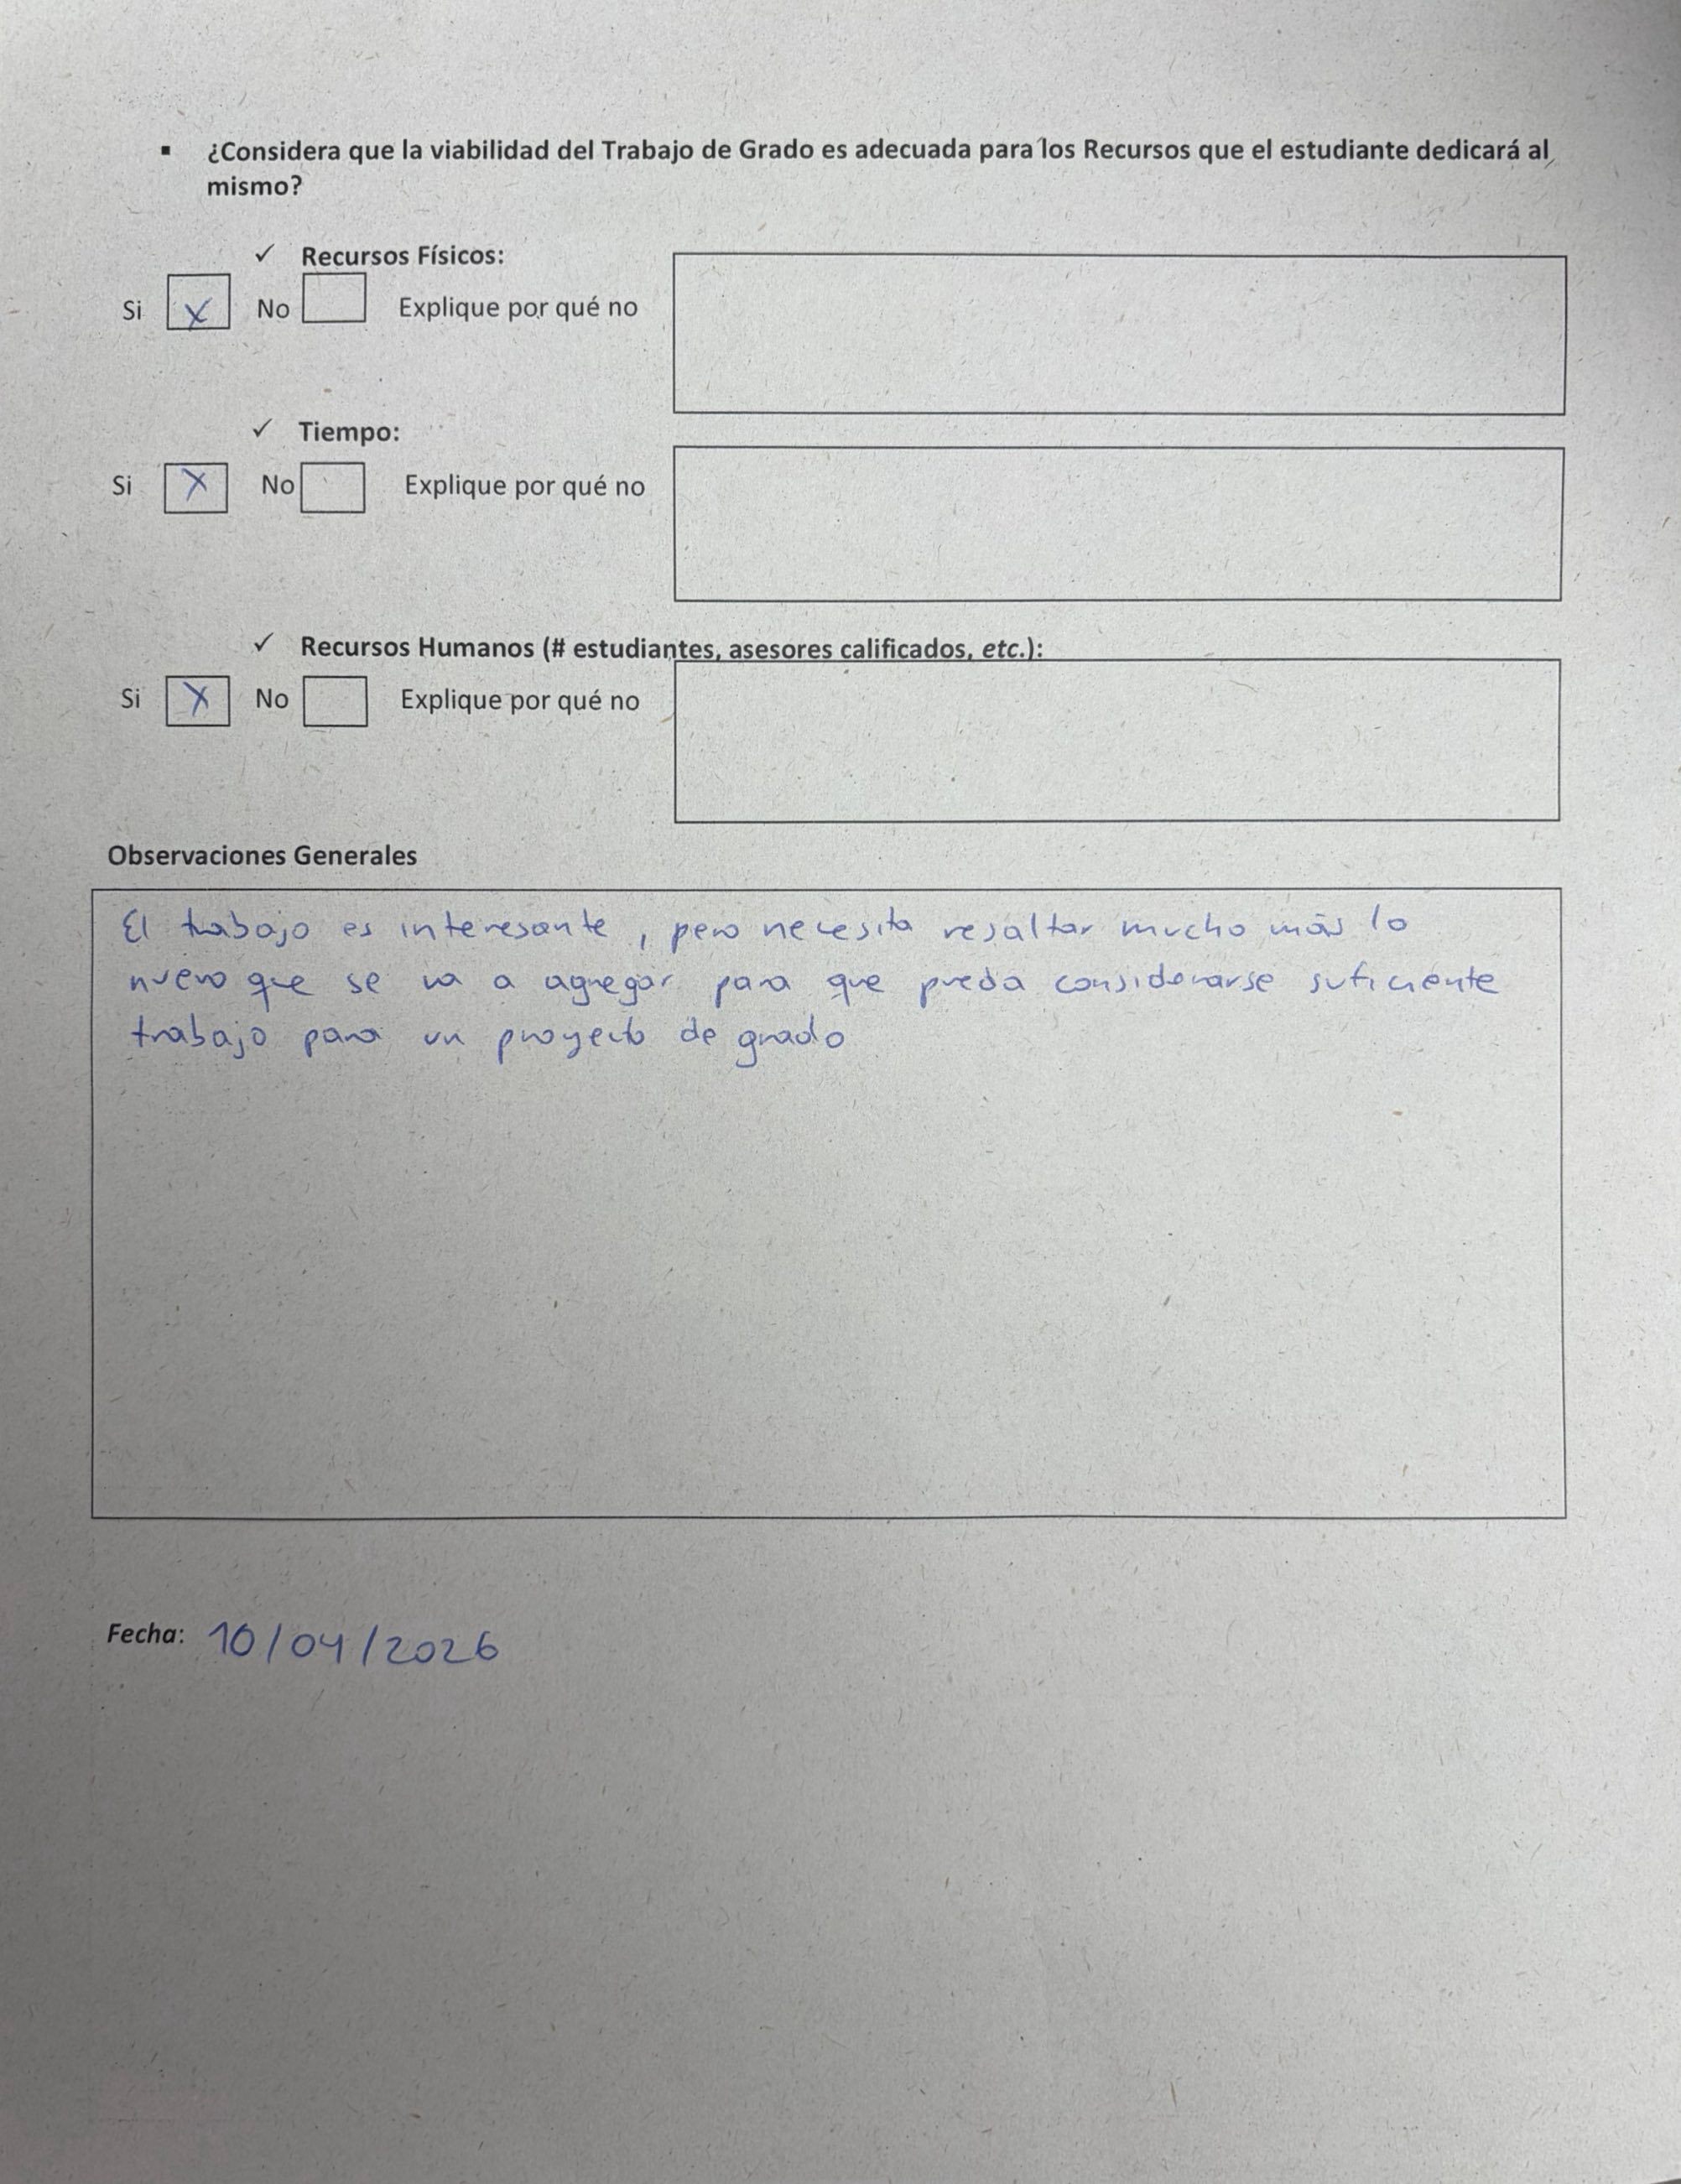
\includegraphics[width=0.9\linewidth]{andrea 2.png}
    \caption{Caption}
    \label{fig:andrea2}
\end{figure}

\textbf{\textcolor{darkblue}{Respuesta (viabilidad y observaciones generales):}}\\[6pt]

\textbf{Recursos Físicos:} Entendemos que los recursos físicos se consideran adecuados. Nos aseguraremos de mantener un inventario claro de los mismos en el documento final.\\[4pt]

\textbf{Tiempo y Recursos Humanos:} Reconocemos las preocupaciones señaladas sobre la viabilidad temporal y el equipo humano. Revisaremos el cronograma y especificaremos con mayor detalle los roles y compromisos de cada integrante del equipo.\\[4pt]

\textbf{Observación general:} Aceptamos la observación de que el trabajo requiere resaltar con mayor claridad el valor nuevo que aporta. Trabajaremos en fortalecer la justificación de la novedad del proyecto para que sea evidente su suficiencia como trabajo de grado.

\newpage

% =============================================
\section{Comentarios 2: Aupelo Carrillo}
% =============================================

\begin{figure}[H]
    \centering
    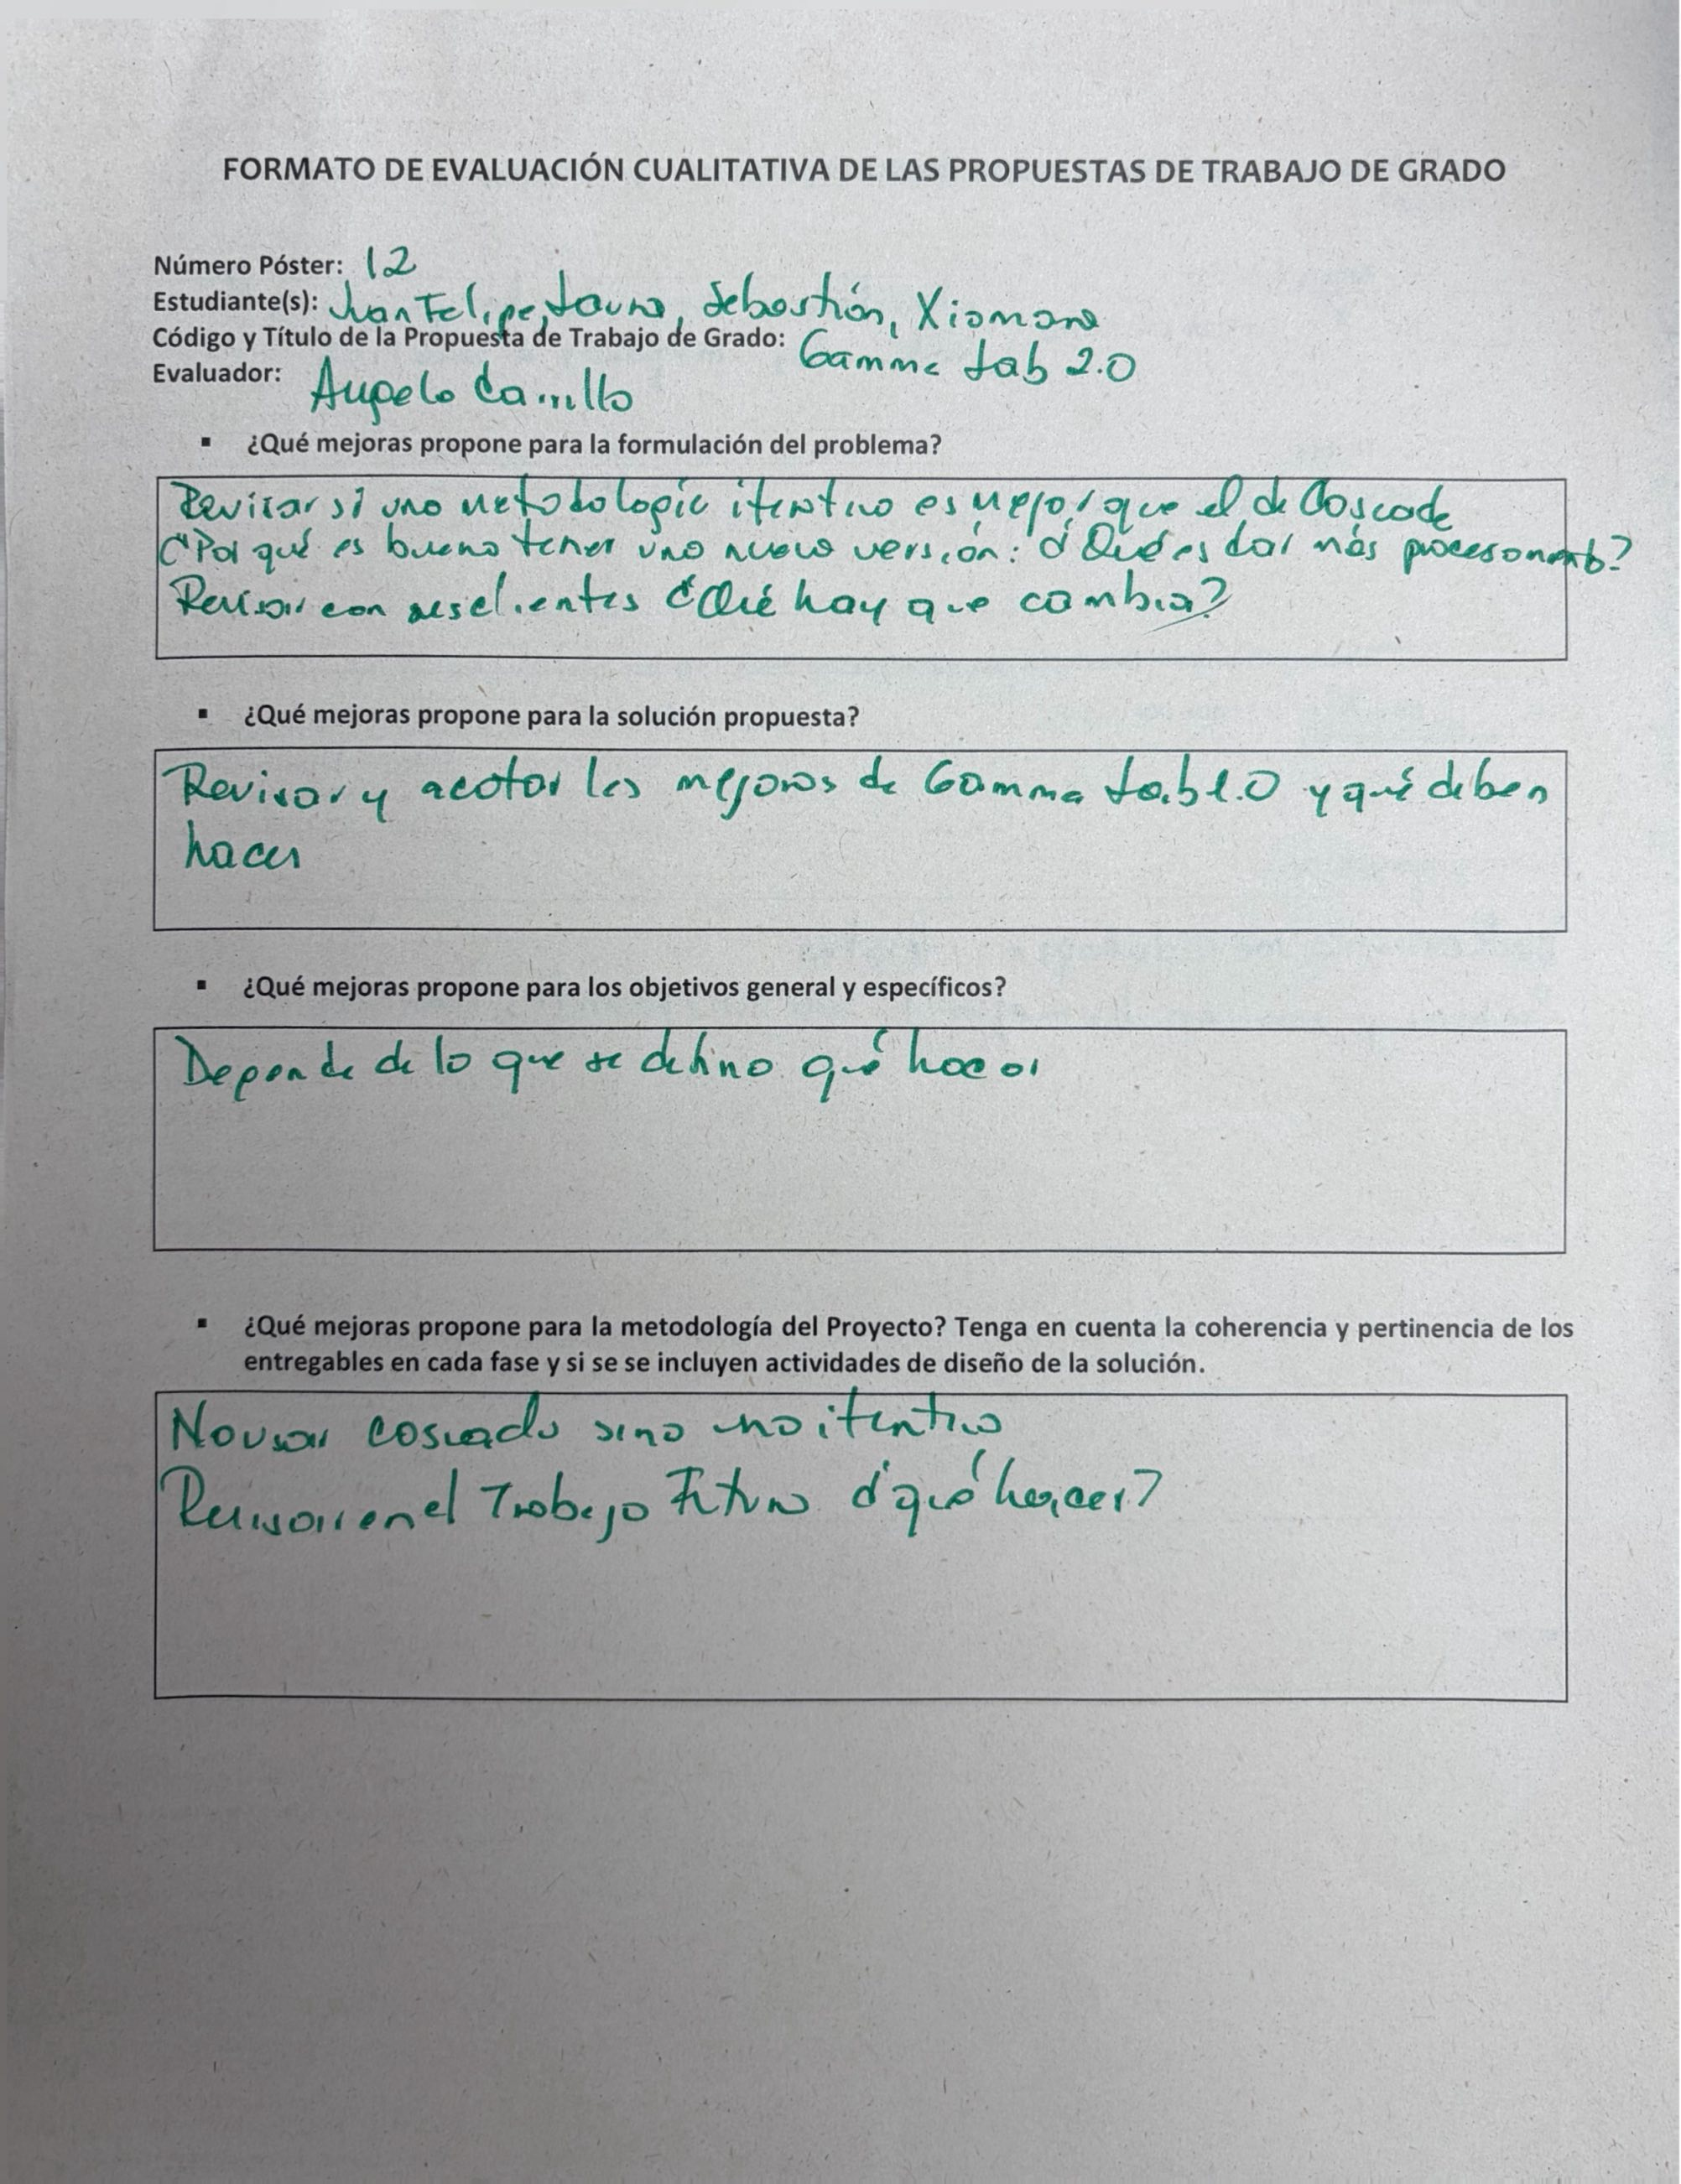
\includegraphics[width=0.9\linewidth]{carrillo 1.png}
    \caption{Caption}
    \label{fig:carrillo1}
\end{figure}

\textbf{\textcolor{darkblue}{Respuesta a los comentarios de Aupelo Carrillo:}}\\[6pt]

\textbf{Formulación del problema:} Agradecemos la sugerencia de revisar si la metodología iterativa es la más adecuada y de justificar con mayor claridad por qué se propone una nueva versión frente a lo existente. Incluiremos una comparación explícita con antecedentes relevantes y argumentaremos con solidez la necesidad del enfoque propuesto.\\[4pt]

\textbf{Solución propuesta:} Aceptamos la recomendación de revisar y adoptar las mejoras de GammaTab 2.0. Incorporaremos un análisis de dichas mejoras y explicaremos cuáles serán integradas y cuáles se abordarán de manera diferente en nuestra propuesta.\\[4pt]

\textbf{Objetivos general y específicos:} Entendemos que los objetivos deben definirse con mayor claridad en función de lo que realmente se va a desarrollar. Reescribiremos el objetivo general para que reflejen con precisión el alcance y los entregables del proyecto.\\[4pt]

\textbf{Metodología:} Reconocemos la observación sobre la necesidad de mayor intencionalidad en la metodología. Revisaremos el Trabajo Futuro y lo articularemos de manera que quede claro qué se hará en el marco de este proyecto y qué quedará como trabajo posterior.

\begin{figure}[H]
    \centering
    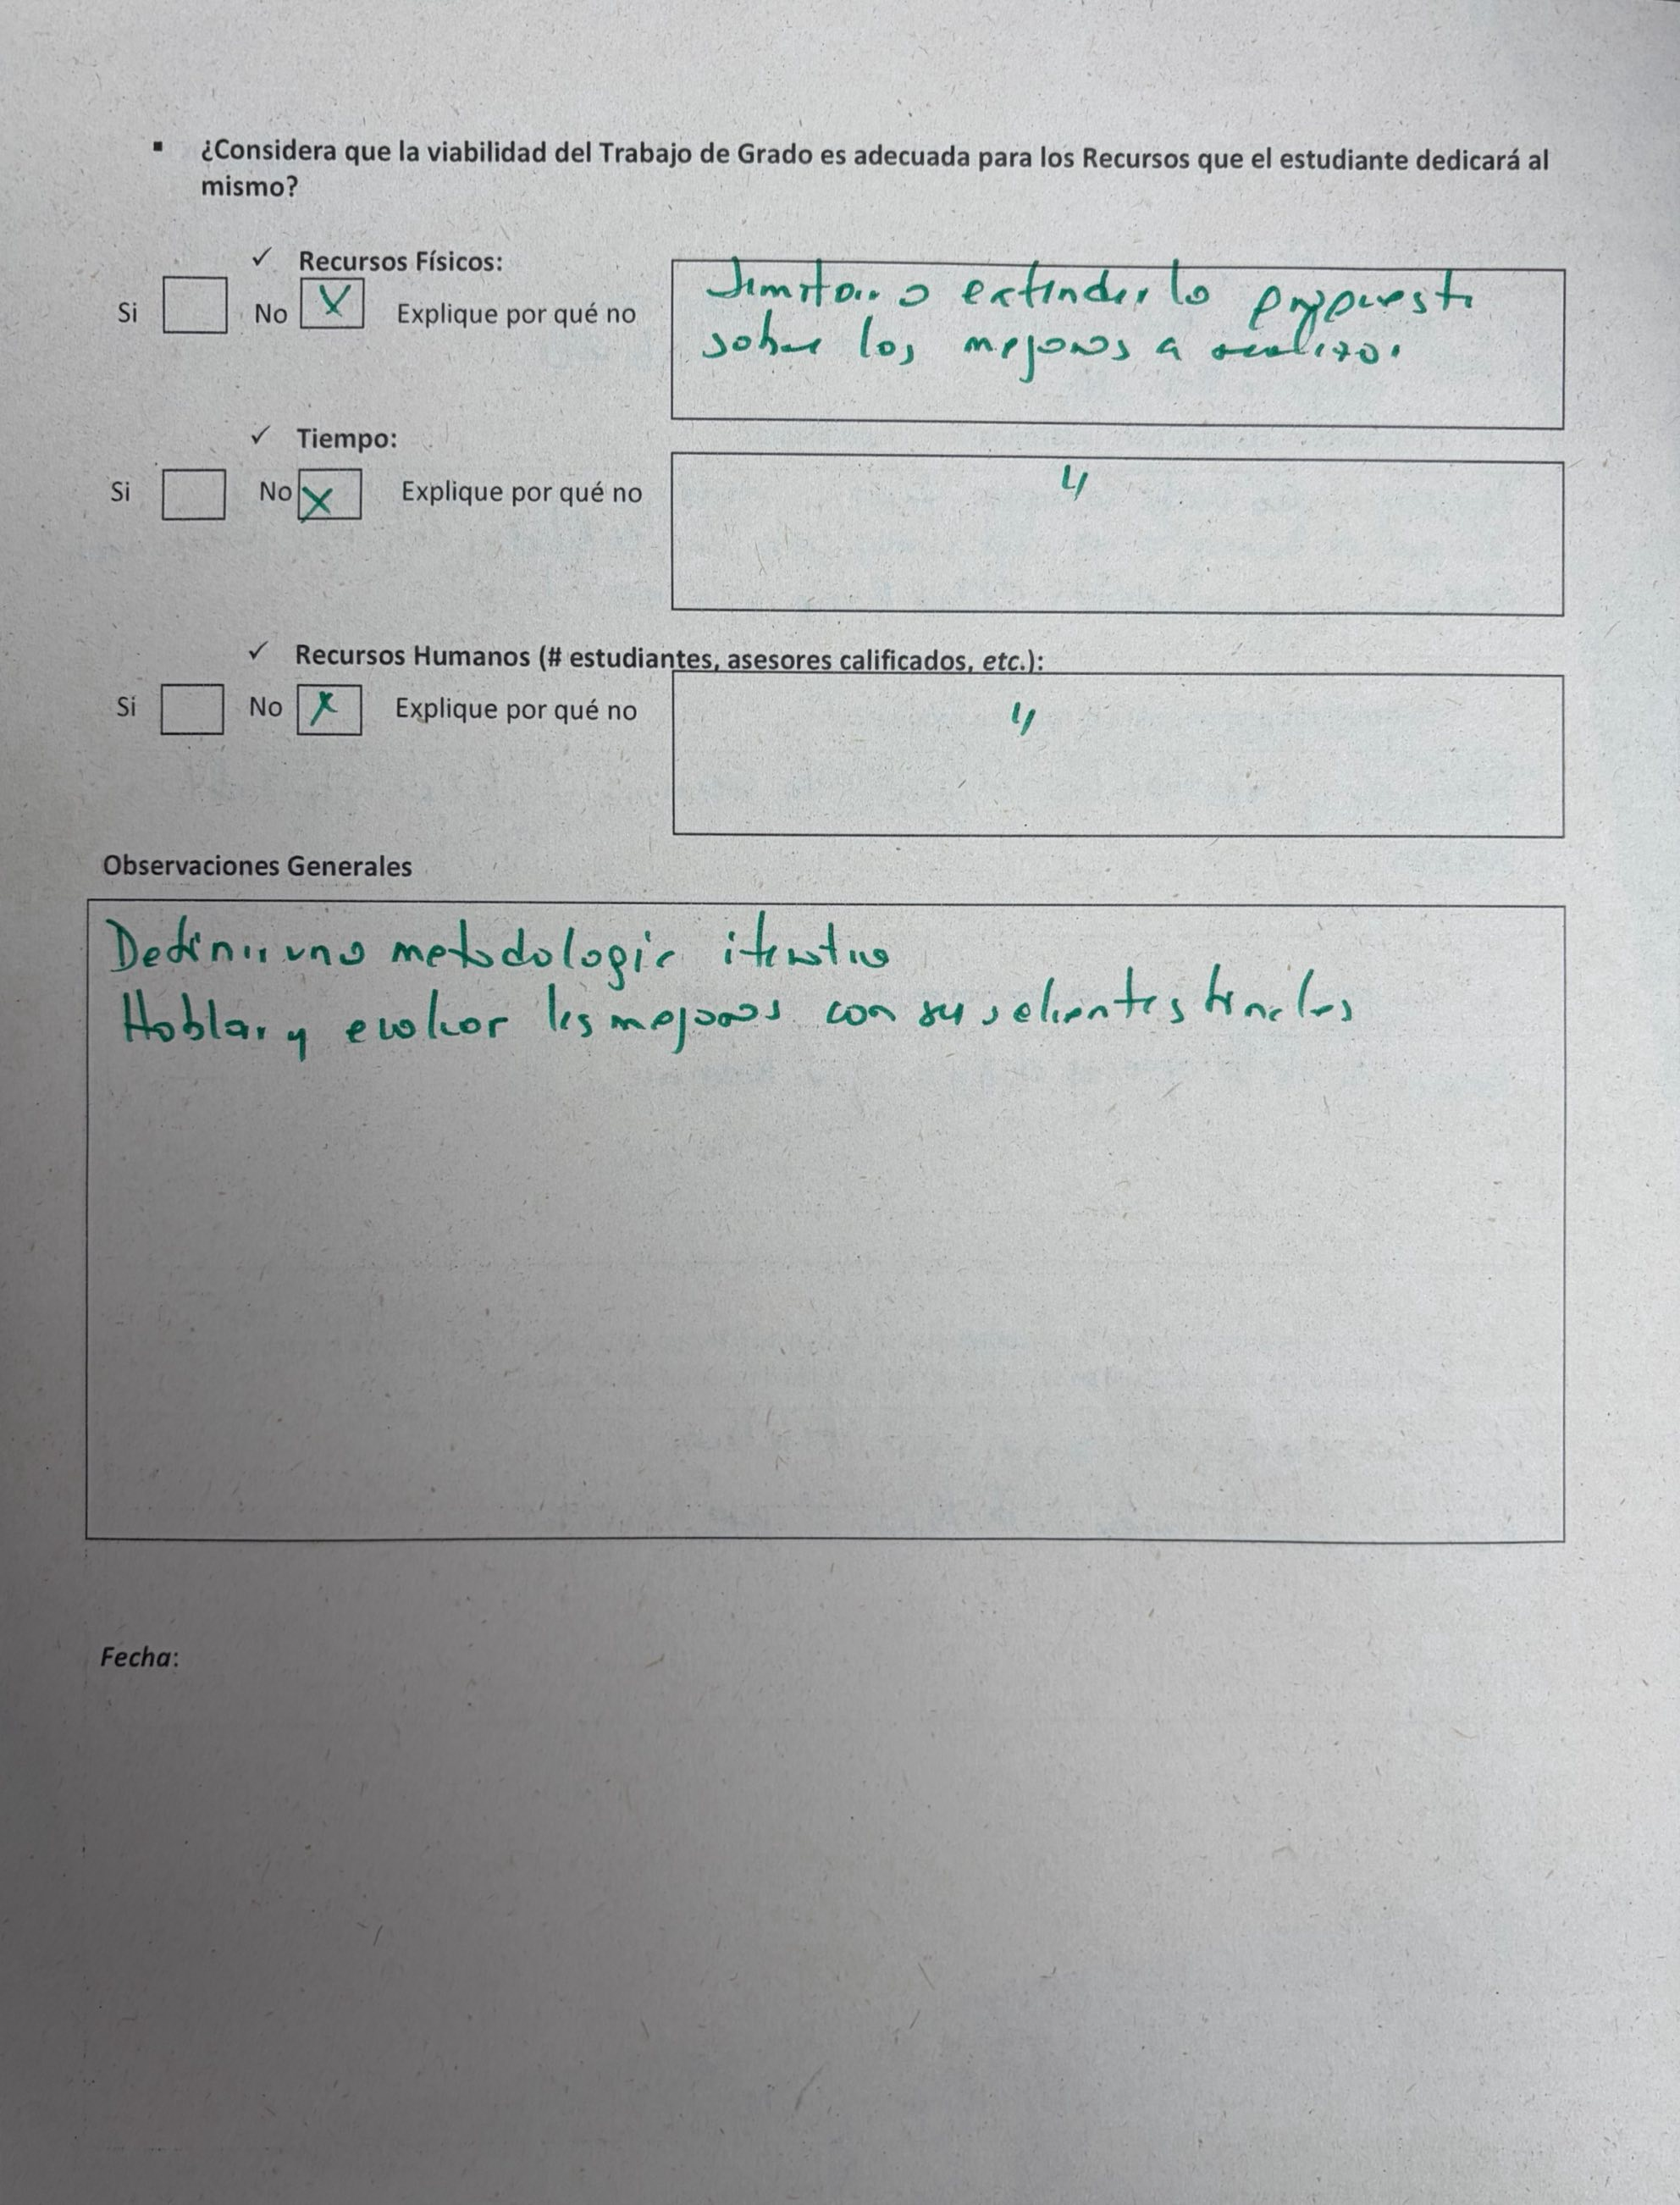
\includegraphics[width=0.9\linewidth]{carrillo 2.png}
    \caption{Caption}
    \label{fig:carrillo2}
\end{figure}

\textbf{\textcolor{darkblue}{Respuesta (viabilidad y observaciones generales):}}\\[6pt]

\textbf{Recursos Físicos:} Agradecemos la indicación de que se debe limitar o clarificar la propuesta en función de las mejoras realizables. Ajustaremos el alcance para que sea coherente con los recursos físicos disponibles.\\[4pt]

\textbf{Tiempo y Recursos Humanos:} Tomamos nota de las preocupaciones sobre la viabilidad temporal y la disponibilidad de recursos humanos calificados. Revisaremos el plan de trabajo para garantizar su factibilidad dentro del tiempo disponible.\\[4pt]

\textbf{Observación general:} Aceptamos la recomendación de definir una metodología más iterativa y de involucrar a los usuarios finales en la evaluación de mejoras. Incorporaremos sesiones de validación con clientes o usuarios reales como parte del proceso metodológico.

\newpage

% =============================================
\section{Comentarios 3: Oman Palacios}
% =============================================

\begin{figure}[H]
    \centering
    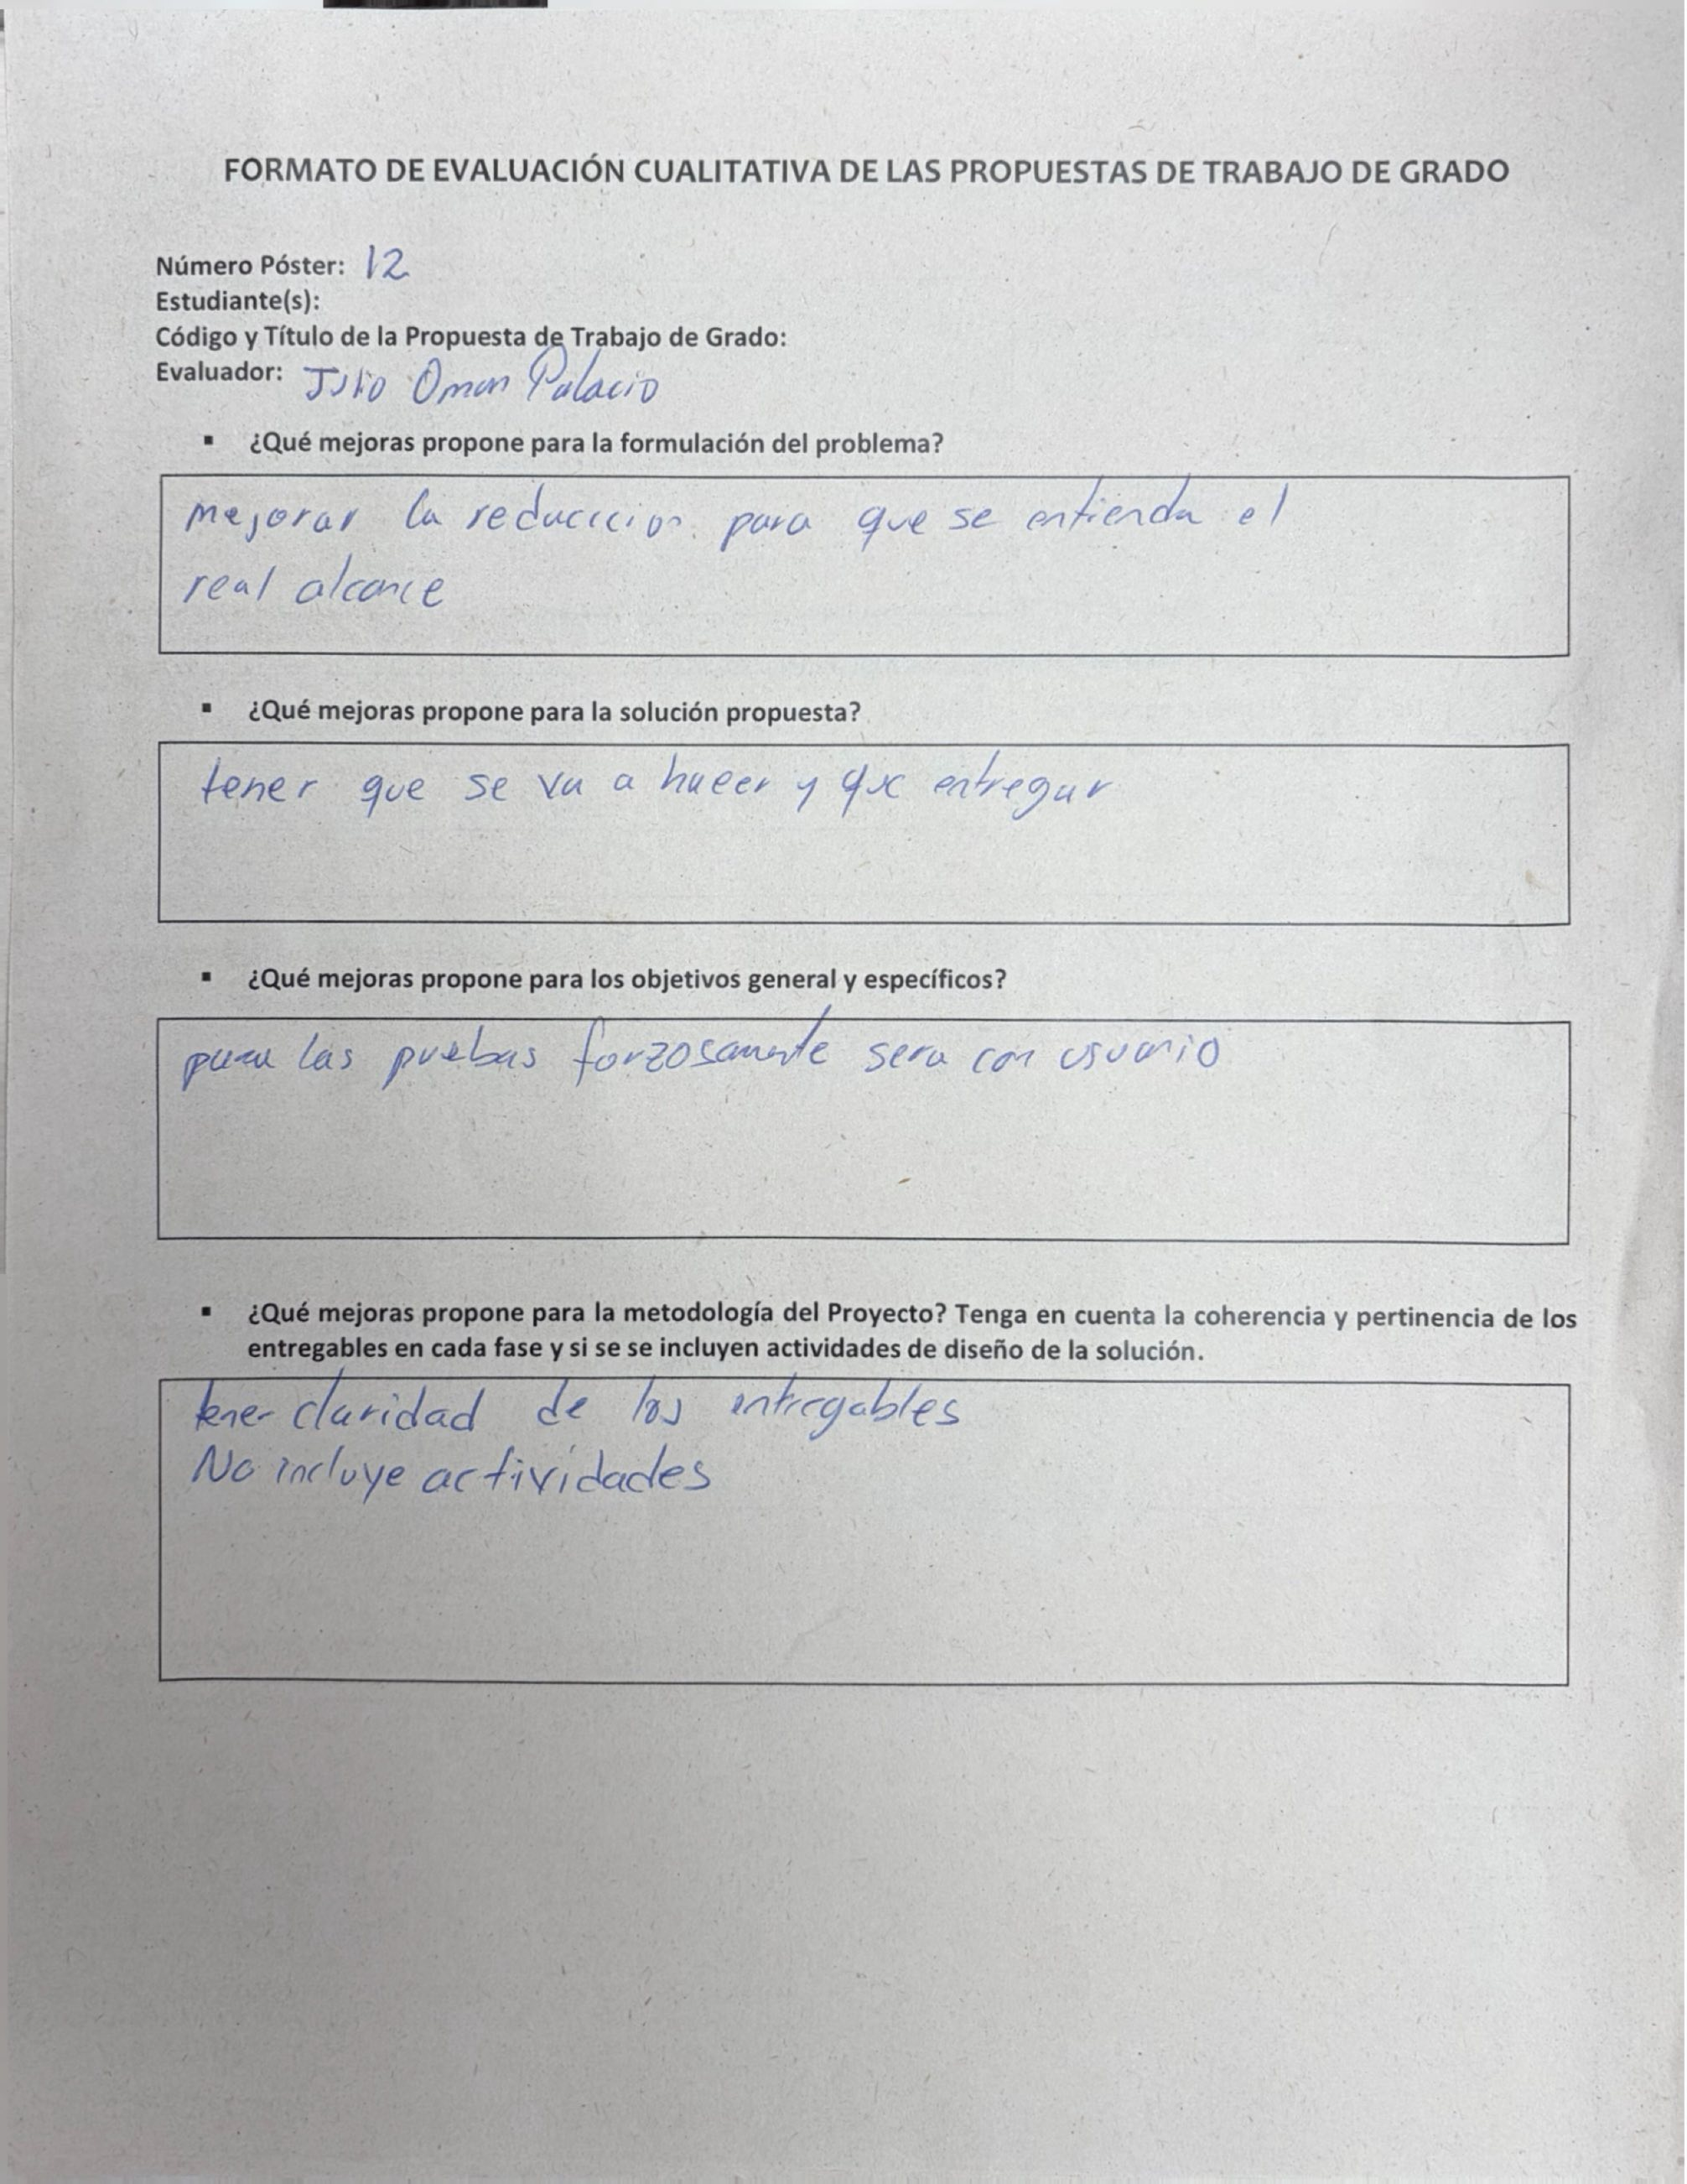
\includegraphics[width=0.9\linewidth]{oman palacios 1.png}
    \caption{Caption}
    \label{fig:oman1}
\end{figure}

\textbf{\textcolor{darkblue}{Respuesta a los comentarios de Omar Palacios:}}\\[6pt]

\textbf{Formulación del problema:} Agradecemos la observación sobre el alcance. Mejoraremos la redacción de esta sección para que el lector comprenda con claridad cuál es el alcance real del proyecto, evitando ambigüedades entre lo que se propone y lo que efectivamente se desarrollará.\\[4pt]

\textbf{Solución propuesta:} Aceptamos la sugerencia. Describiremos de forma más concreta y detallada qué se va a construir y qué entregables concretos se producirán al final del proyecto.\\[4pt]

\textbf{Objetivos general y específicos:} Entendemos que las pruebas deben involucrar forzosamente a usuarios reales. Incorporaremos objetivos específicos relacionados con la validación con usuarios y ajustaremos el diseño de pruebas en consecuencia.\\[4pt]

\textbf{Metodología:} Aceptamos las dos observaciones: mejoraremos la claridad de los entregables en cada fase e incluiremos actividades de diseño de la solución que actualmente no están contempladas de manera explícita.

\begin{figure}[H]
    \centering
    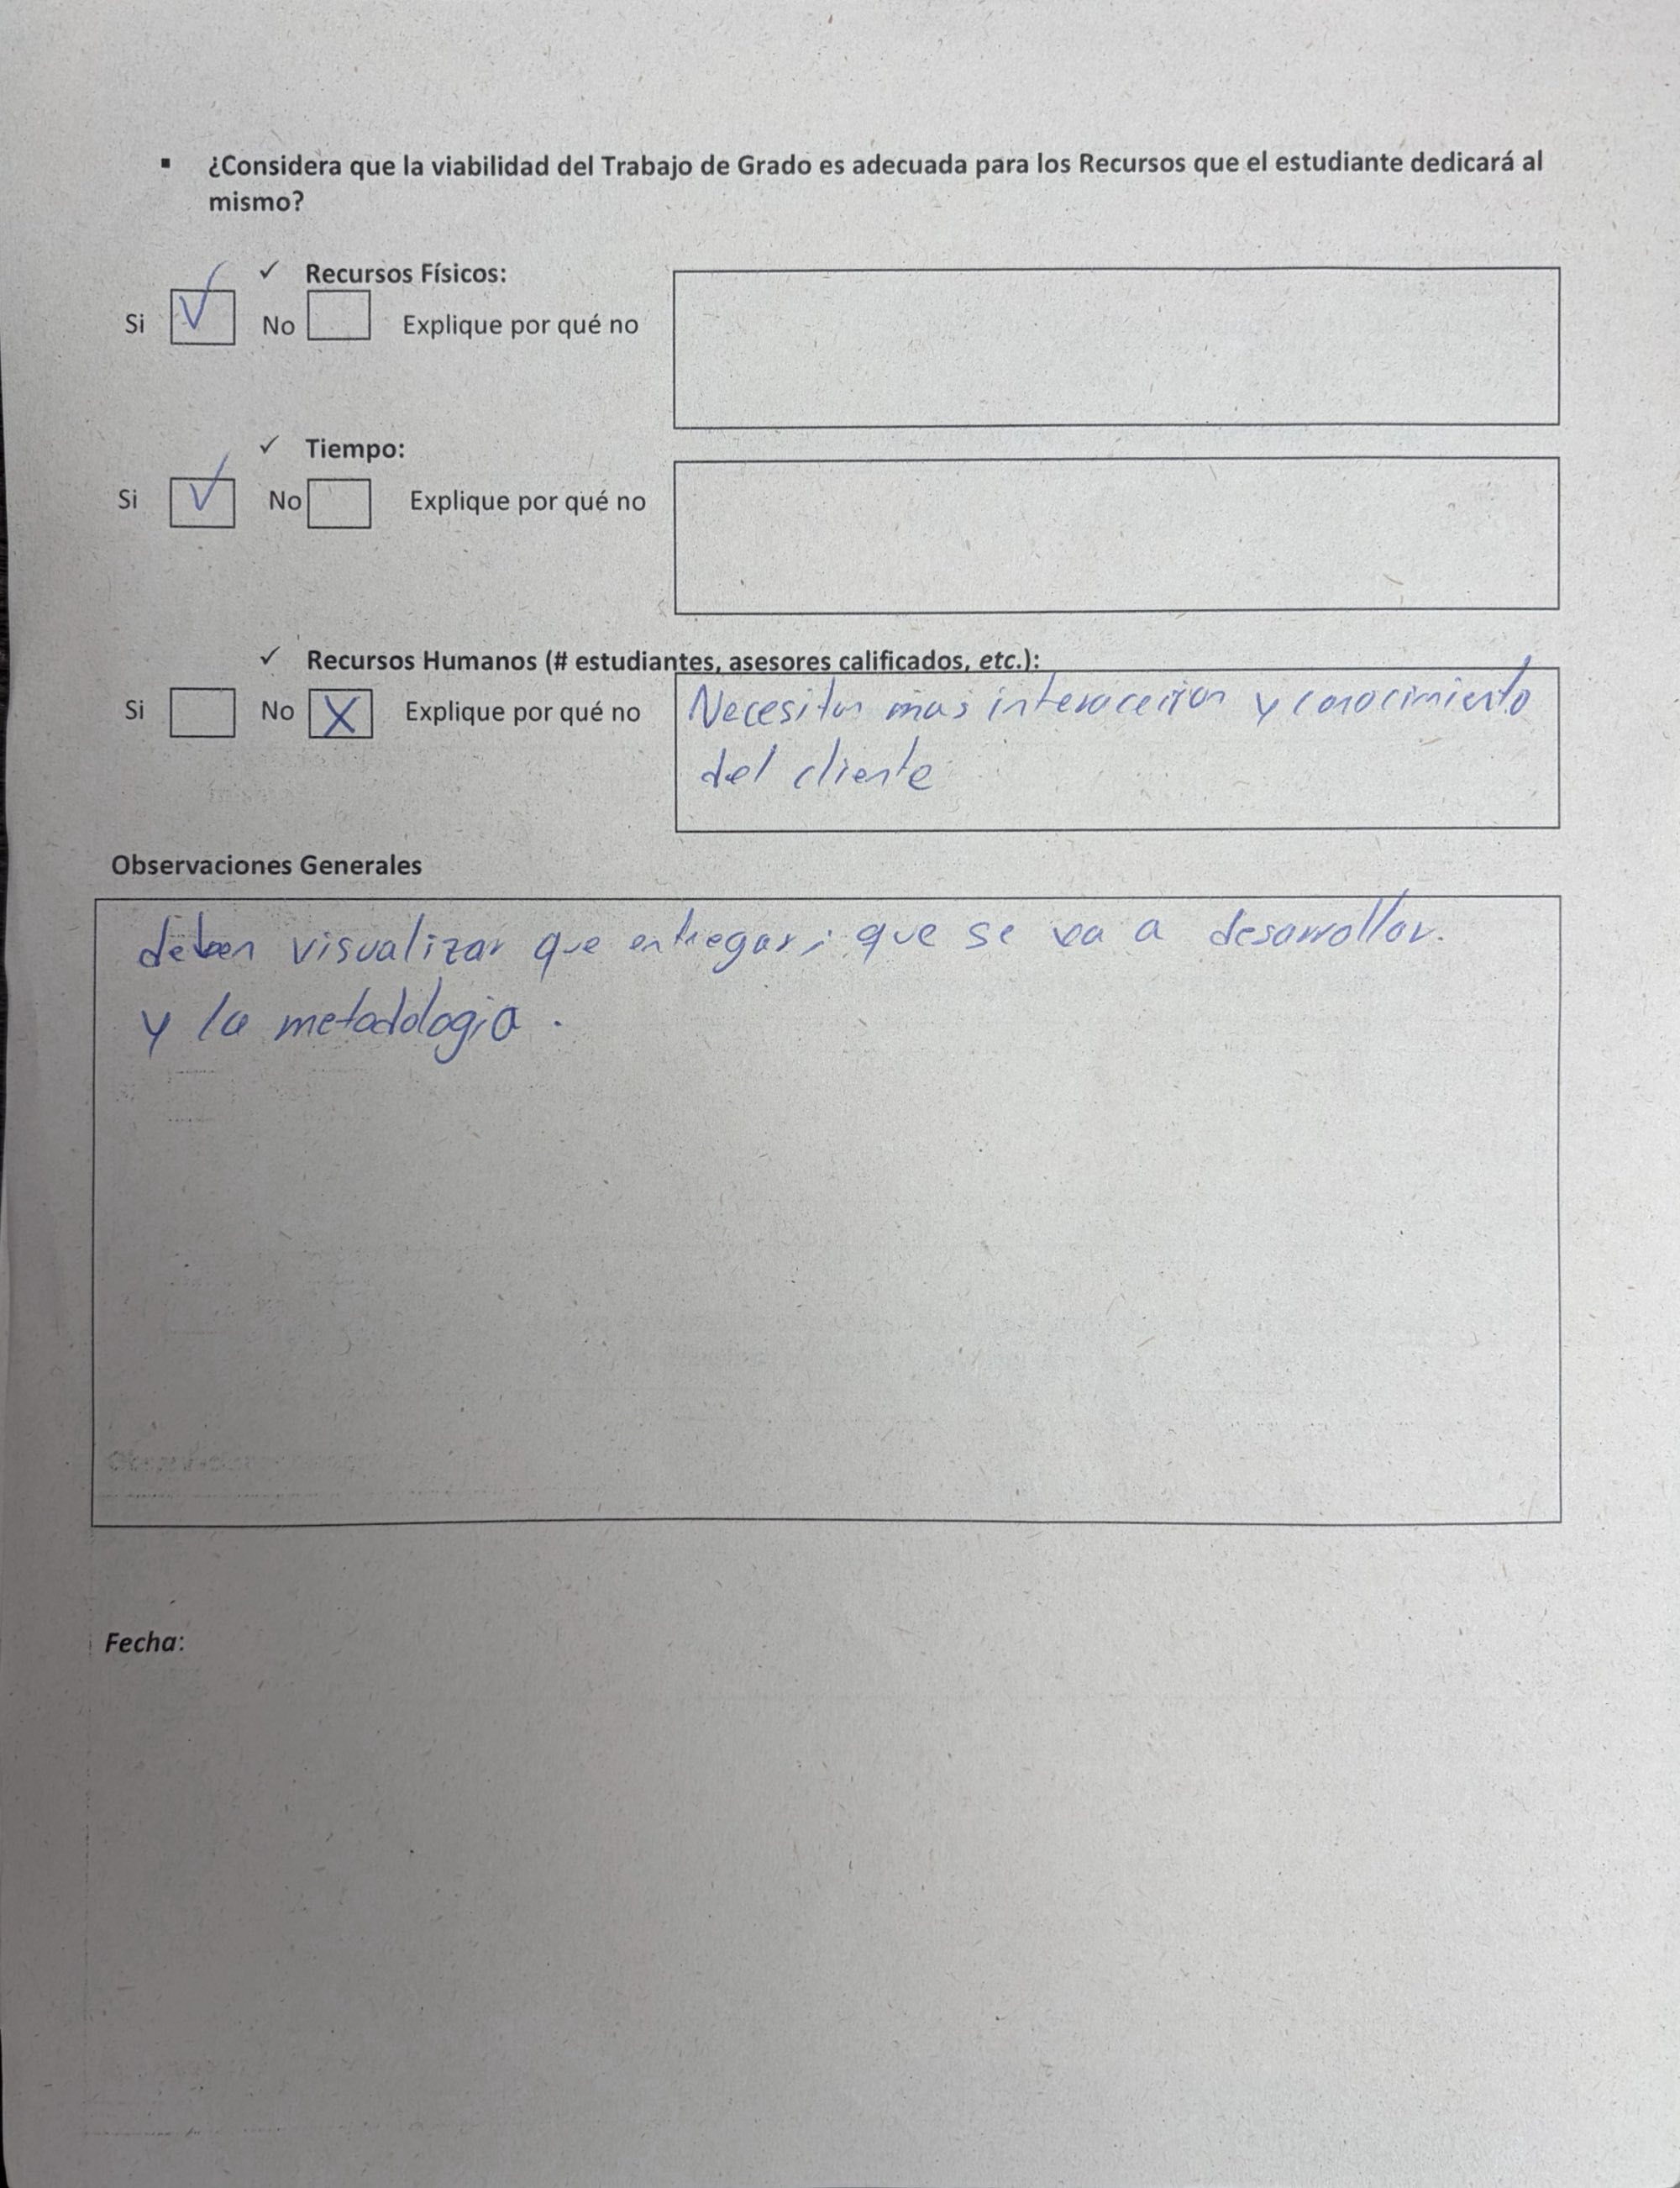
\includegraphics[width=0.9\linewidth]{oman palacios 2.png}
    \caption{Caption}
    \label{fig:oman2}
\end{figure}

\textbf{\textcolor{darkblue}{Respuesta (viabilidad y observaciones generales):}}\\[6pt]

\textbf{Recursos Físicos y Tiempo:} Agradecemos la valoración positiva sobre la viabilidad en estos aspectos. Mantendremos el enfoque actual y garantizaremos que el plan de uso de recursos esté bien documentado.\\[4pt]

\textbf{Recursos Humanos:} Reconocemos que se requiere mayor interacción con el cliente y un conocimiento más profundo de su contexto. Planificaremos sesiones de acercamiento con los usuarios para fortalecer el entendimiento del dominio del problema.\\[4pt]

\textbf{Observación general:} Aceptamos plenamente la recomendación de visualizar con mayor claridad los entregables y la metodología de desarrollo. Incluiremos diagramas, tablas de entregables por fase y una descripción más detallada del proceso para facilitar su comprensión.

\end{document}